\documentclass[10pt,aspectratio=169]{beamer}
\usetheme{ffloyd}
\usepackage{amsmath,amssymb,booktabs}
\usefonttheme[onlymath]{serif}
\setmainfont{Latin Modern Roman}
\ifdefstring{\ffloydbackground}{white}{%
  \graphicspath{{figures/white/}}%
}{%
  \ifdefstring{\ffloydbackground}{softcream}{%
    \graphicspath{{figures/softcream/}}%
  }{\graphicspath{{figures/}}}%
}

\title{Evidence, in warm color}
\subtitle{A Metropolis theme in the ffloyd palette}
\author{An illustrative research presentation}
\date{October 2026}
\setbeamertemplate{frame footer}{\textsc{ffloyd / metropolis}}

\newcommand{\chartnote}[1]{\par\vspace{-0.2em}{\scriptsize #1\hfill Synthetic data; illustrative only.}}
\newcommand{\swatch}[2]{%
  \begin{minipage}[t]{0.112\textwidth}\centering
    {\color{#1}\rule{\linewidth}{0.55cm}}\par
    \vspace{0.15em}{\scriptsize #2}
  \end{minipage}\hfill}

\begin{document}

\maketitle

\begin{frame}{A quiet background. A clear visual hierarchy.}
  \ifdefstring{\ffloydbackground}{white}{Soft white}{%
    \ifdefstring{\ffloydbackground}{softcream}{Soft cream}{Warm cream}}
  gives the page its tone. Deep blue anchors the structure.
  \alert{Golden yellow draws attention}; jade green marks examples.

  \vspace{1em}
  \swatch{ff_yellow}{Gold}
  \swatch{ff_green}{Jade}
  \swatch{ff_blue}{Blue}
  \swatch{ff_terracotta}{Terracotta}
  \swatch{ff_violet}{Violet}
  \swatch{ff_rose}{Rose}
  \swatch{ff_olive}{Olive}
  \swatch{ff_deep_blue}{Deep blue}

  \vspace{1.2em}
  \begin{description}
    \item[Categorical] Distinguish groups without implying rank.
    \item[Sequential] Let darker values indicate more.
    \item[Diverging] Compare departures on either side of a reference.
  \end{description}
\end{frame}

\section{Ideas and notation}

\begin{frame}{From a research question to a measurement}
  \begin{columns}[T,onlytextwidth]
    \begin{column}{0.48\textwidth}
      \textbf{What would we want to know?}
      \begin{itemize}
        \item Who uses each transport mode?
        \item How does service change over time?
          \begin{itemize}
            \item Compare districts consistently.
            \item Keep the measurement scale fixed.
          \end{itemize}
        \item Which areas improve or decline?
      \end{itemize}
    \end{column}
    \begin{column}{0.46\textwidth}
      \textbf{A simple analytical workflow}
      \begin{enumerate}
        \item Define an outcome and population.
        \item Establish a meaningful baseline.
        \item Estimate the change and uncertainty.
        \item \alert{Separate evidence from interpretation.}
      \end{enumerate}
    \end{column}
  \end{columns}
  \vspace{0.8em}
  {\small All examples in this deck describe a fictional mobility study.}
\end{frame}

\begin{frame}{Mathematics with a focused accent}
  Let $Y_i(d)$ denote a potential outcome and $D_i\in\{0,1\}$ treatment status.
  The average treatment effect is
  \[
    \alert{\tau}=\mathbb{E}\!\left[Y_i(1)-Y_i(0)\right].
  \]
  A working regression and its least-squares estimate are
  \begin{align*}
    Y_i &= \alpha + \alert{\tau}D_i + \mathbf{x}_i^{\mathsf T}\boldsymbol{\beta}
           + \varepsilon_i, \\
    \widehat{\boldsymbol{\theta}}
      &= \underset{\boldsymbol{\theta}}{\operatorname{arg\,min}}\;
         \sum_{i=1}^{n}\bigl(Y_i-\mathbf{z}_i^{\mathsf T}\boldsymbol{\theta}\bigr)^2.
  \end{align*}
  \begin{exampleblock}{Interpretation}
    Under random assignment and the relevant causal assumptions,
    $\widehat{\tau}$ estimates the average effect of treatment.
  \end{exampleblock}
\end{frame}

\begin{frame}{Blocks, examples, and alerts}
  \begin{block}{Main result}
    Put the claim and its scope together. Use the blue block for definitions,
    propositions, or a result the audience should retain.
  \end{block}
  \begin{alertblock}{A qualification that matters}
    \alert{An association alone does not establish causation.}
    Gold highlights the point while the supporting text stays blue.
  \end{alertblock}
  \begin{exampleblock}{A concrete example}
    Compare the same outcome across two randomly assigned groups,
    then report an estimate alongside its uncertainty.
  \end{exampleblock}
\end{frame}

\section{Three views of the data}

\begin{frame}{Categorical: different modes, distinct identities}
  \small A fictional survey records the main mode used for each trip.\par
  \normalsize
  \vspace{0.25em}
  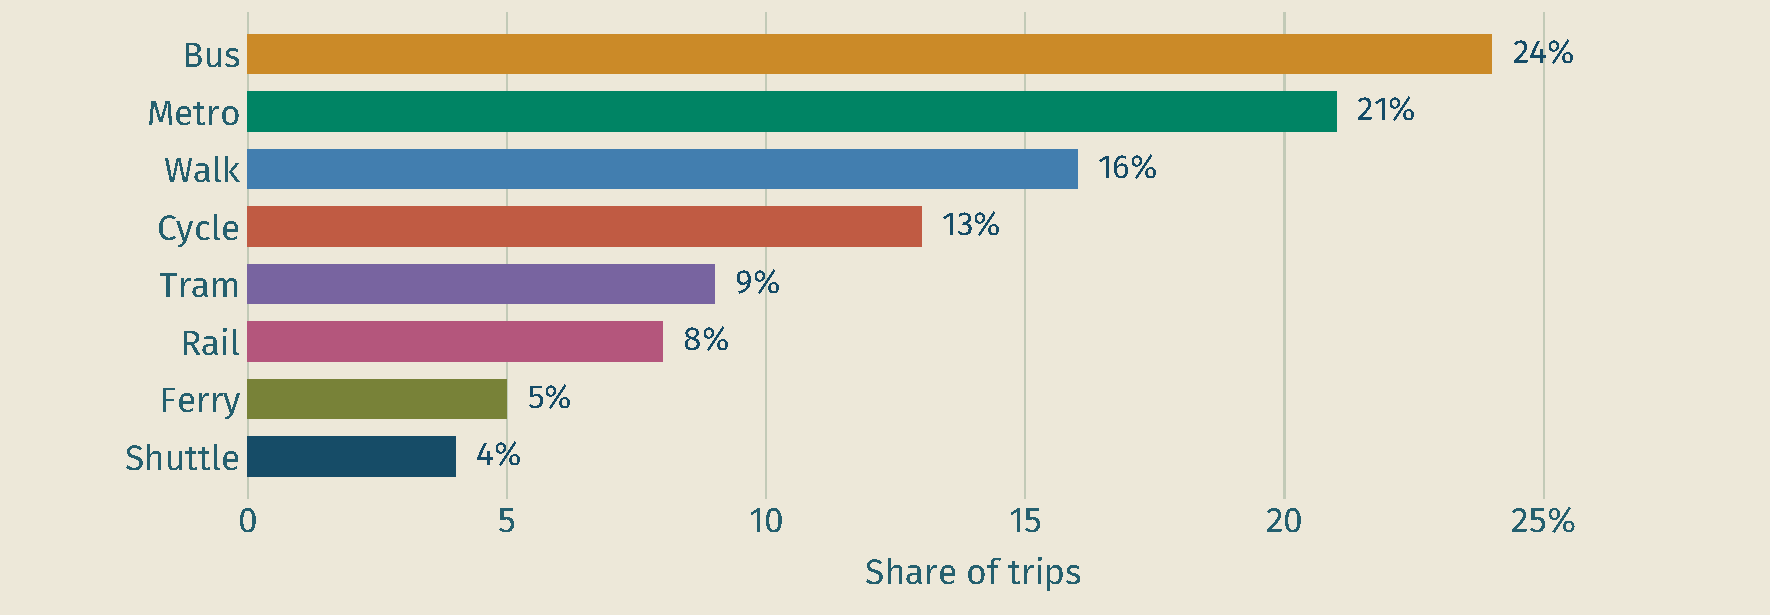
\includegraphics[width=\textwidth]{categorical.pdf}
  \chartnote{Eight categories; the complete categorical palette.}
\end{frame}

\begin{frame}{Sequential: service builds over time}
  \small Availability index: 0 means least service; 100 means most service.\par
  \normalsize
  \vspace{0.25em}
  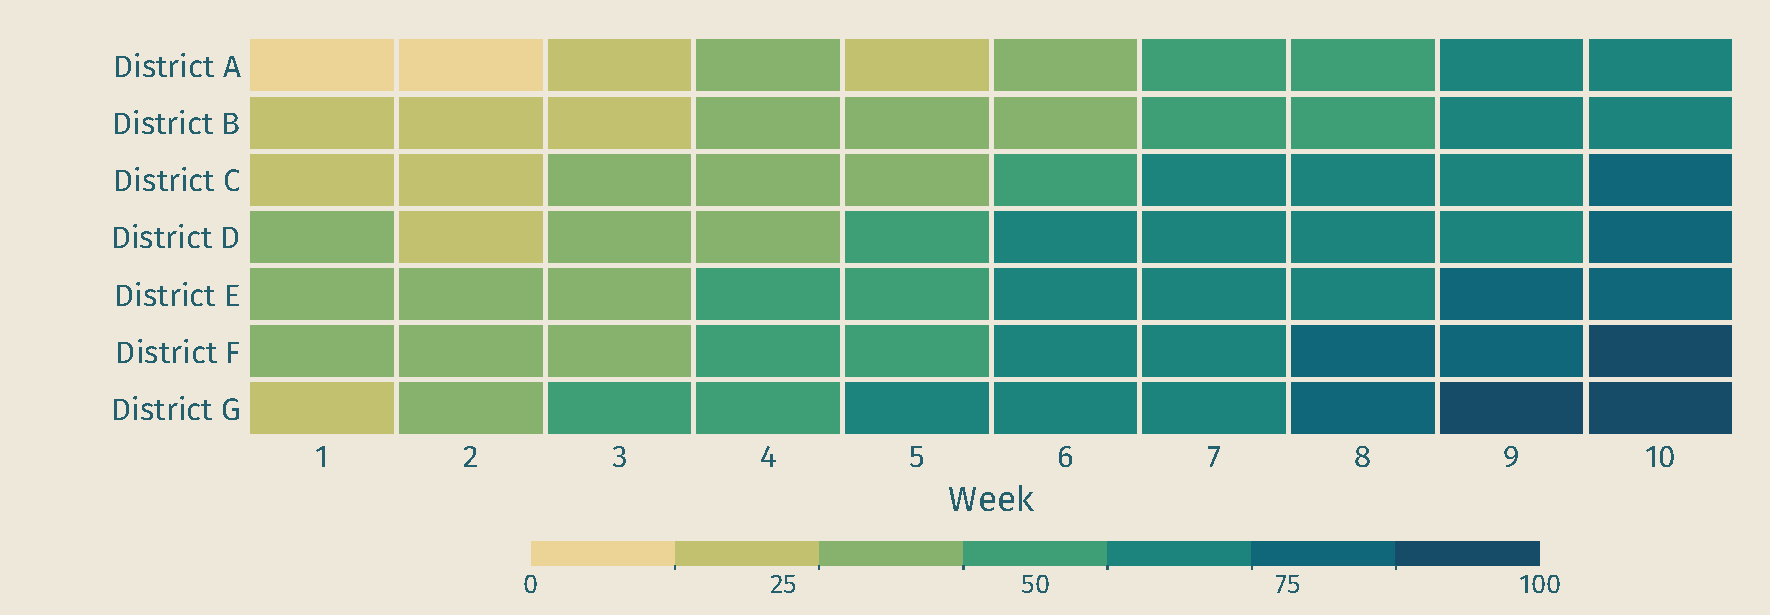
\includegraphics[width=\textwidth]{sequential.pdf}
  \chartnote{Seven ordered colors; a common 0--100 scale across every district.}
\end{frame}

\begin{frame}{Diverging: changes on either side of zero}
  \small Differences in satisfaction relative to the baseline, by service area.\par
  \normalsize
  \vspace{0.25em}
  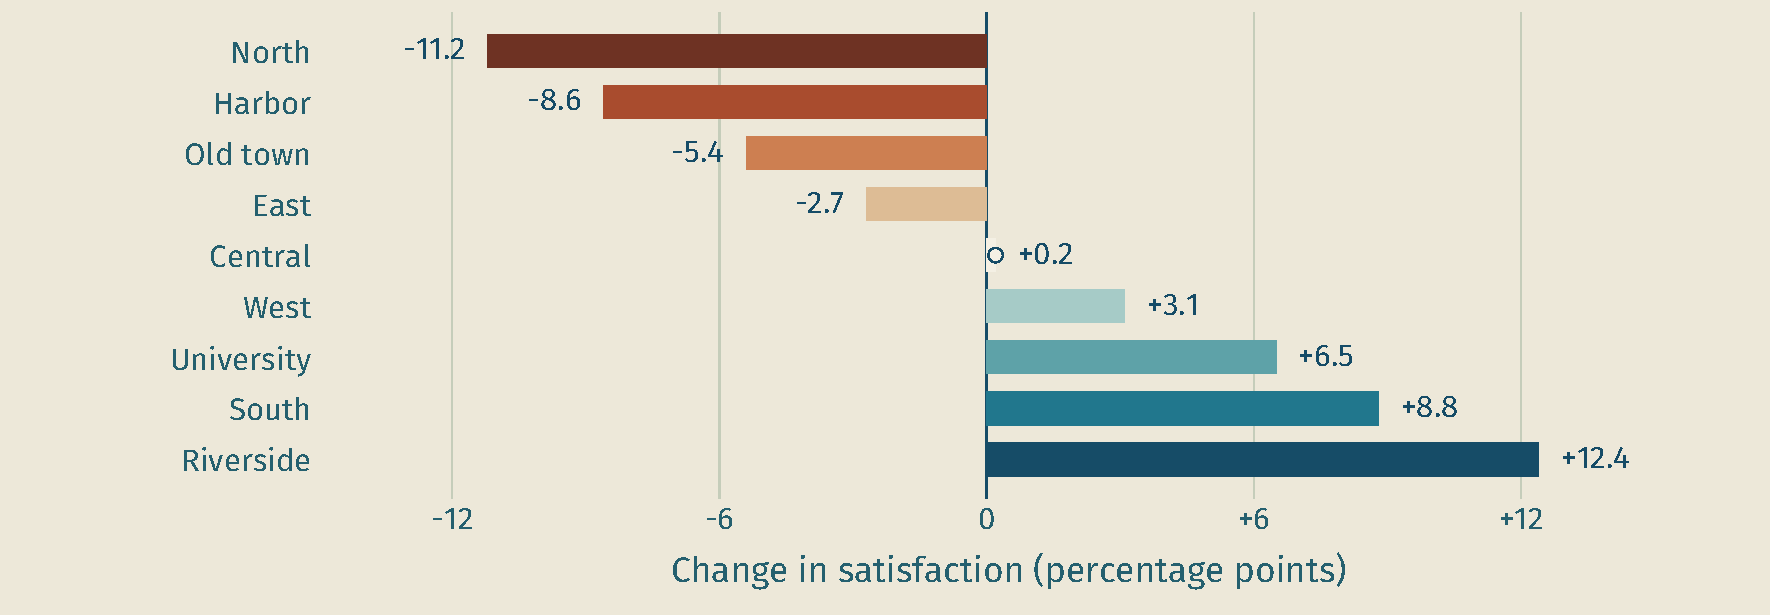
\includegraphics[width=\textwidth]{diverging.pdf}
  \chartnote{Nine colors centered on zero; warm below, cool above.}
\end{frame}

\begin{frame}{A compact result table}
  \begin{columns}[T,onlytextwidth]
    \begin{column}{0.56\textwidth}
      \begin{tabular}{@{}lrr@{}}
        \toprule
        \textbf{Area} & \textbf{Change} & \textbf{95\% interval} \\
        \midrule
        North      & $-11.2$ & $[-14.6,-7.8]$ \\
        Central    & $+0.2$  & $[-2.1,+2.5]$ \\
        Riverside  & $+12.4$ & $[+8.9,+15.9]$ \\
        \bottomrule
      \end{tabular}
      \vspace{0.5em}

      {\scriptsize Synthetic estimates and intervals; percentage points.}
    \end{column}
    \begin{column}{0.39\textwidth}
      \textbf{Read the estimate with its uncertainty.}
      \begin{itemize}
        \item Report the unit and reference.
        \item Show the interval with the point estimate.
        \item \alert{Near zero can still be informative.}
      \end{itemize}
    \end{column}
  \end{columns}
\end{frame}

\begin{frame}[fragile]{Use the theme in your next deck}
\begin{verbatim}
\documentclass[aspectratio=169]{beamer}
\usetheme{ffloyd} % cream by default
% Or: \usetheme[background=white]{ffloyd}
% Or: \usetheme[background=softcream]{ffloyd}

% Inside your slides:
\alert{An important point}
\textcolor{ff_green}{An example}
\end{verbatim}
  {\small Keep the two theme files and \texttt{ffloyd\_colors.tex} with your deck.
  Compile with LuaLaTeX for Metropolis's Fira typography.}
  \vspace{0.5em}

  {\scriptsize Based on \href{https://github.com/matze/mtheme}{Metropolis by Matthias Vogelgesang and contributors}.
  Theme adaptation: CC BY-SA 4.0.}
\end{frame}

\begin{frame}[standout]
  Keep the evidence clear.\par
  \vspace{0.4em}
  Give the important point \alert{a little gold}.
\end{frame}

\end{document}
